% !TeX encoding = UTF-8
% !TeX spellcheck = en_US
% !TeX root = ../MasterThesis_OlivierChurlaud_2016.tex

\chapter{System and correction simulation}
One difficulty in improving the current correction process is that machine time is expensive: tests cannot be done very often. A wrong correction can indeed destabilize the orbit or worse, lose the electrons in the vacuum chamber walls, and thus it cannot be tested when the storage ring is on service or other scientists do experiments or measurements for their own research. Furthermore, as presented previously, the process is complex and one must be sure that every actor will play correctly in the improvement proposition. Simulating the whole environment is expected to mitigate this problem, and reduce the online experimental time needed during nights and weekends.

Additionally,  Based on theses observations, the 

A short theoretical background will be first presented to introduce the formalism needed to describe control processes. Based on this, the way the system identification was conducted to model the storage ring will be presented. As the study of the correction architecture at BESSY~II showed that some improvements in the correction process were possible, a new architecture of the correction, allowing better results, will be described. Finally the simulation results will be discussed.

\section{Theoretical background}
\subsection{System}
To model a practical process, a system is used. 

A system is defined as an operator $\mathcal{L}$, changing a set of $q$ inputs $\vec{u}$ in into $p$ outputs $\vec{y}$. Generally, the inputs, outputs and operator can vary with time, position, temperature or any possible variable.

For example if the inputs, outputs and operators are only time dependent:
\begin{equation}
	\vec{y}(t) = \mathcal{L}[\vec{u}(t),t]
\end{equation}

\subsection{Linear time invariant system}
A linear time invariant (LTI) system is 
\begin{itemize}
	\item \textbf{time invariant}: the operator $\mathcal{L}$ does not depend on the time, meaning that a given input will always generate the same output: $\mathcal{L}[\vec{u},t]=\mathcal{L}[\vec{u}]$. This is can also being described as
	\begin{equation}
		\vec{y}(t) = \mathcal{L}[\vec{u}(t)] \implies \forall \tau, \quad \vec{y}(t-\tau) = \mathcal{L}[\vec{u}(t-\tau)]
	\end{equation}
	\item \textbf{linear}: 	the operator  $\mathcal{L}$ is linear
	\begin{equation}
		\begin{cases}
			\vec{y}_1(t) = \mathcal{L}[\vec{u}_1(t)] \\
			\vec{y}_2(t) = \mathcal{L}[\vec{u}_2(t)] 
		\end{cases}
		\implies \forall (\alpha, \beta) \in \mathbb{R}^2, \quad
		\alpha \vec{y}_1(t) + \beta \vec{y}_2(t) = \mathcal{L}[\alpha\vec{u}_1(t)+\beta\vec{u}_2(t)]
	\end{equation}
	This linearity property allows analyzing any complicated input as a sum of easier ones that will be superposed. The system complexity can thus be more easily handled.
\end{itemize}

It can be proven that in a LTI system, an harmonic input signal of frequency $f_0$ will produced an harmonic output signal with the same frequency. Only the amplitude and the phase will be different.

\subsection{Transfer function}
LTI systems can be described with specific operators called transfer functions.

Let a system with a single input and single output (SISO) be described as 
\begin{equation}
	\label{eq:controlth_diff_eq}
	\sum\limits_{k=0}^M a_k \frac{d^k y}{dt^k}(t) = \sum\limits_{j=0}^N b_j \frac{d^j u}{dt^j}(t).
\end{equation}
Taking its Laplace transform yields
\begin{equation}
\sum\limits_{k=0}^N a_k s^k Y(s) = \sum\limits_{j=0}^M b_j s^j U(s).
\end{equation}
where a $Y(s) = \mathcal{L}\{y(t)\}$ and $U(s) = \mathcal{L}\{u(t)\}$ the Laplace transform of its output and input.

The transfer function is defined as
\begin{equation}
	\label{eq:controlth_tf}
	G(s) = \frac{Y(s)}{U(s)} = \frac{\sum\limits_{j=0}^M b_j s^j}{\sum\limits_{k=0}^N a_k s^k}.
\end{equation}

\begin{itemize}
	\item $N$ is the order of the system (i.e. the order of the pole polynomial) 
	\item $N-M$ is the relative order
	\item A system $G(s)$ is defined as \emph{proper} if $\lim\limits_{\omega \rightarrow \infty} G(j\omega) = D \neq \infty$, which requires $M < N$. It means that it can be physically realized.
\end{itemize}

\subsection{State-space description}
If transfer functions are a very useful tool (for example to represent the Bode diagram of a function or easily combine successive systems), computing their outputs is not very practical. Another representation is often used, with the help of a inner variable $x(t)$:
\begin{equation}
\begin{cases}
	\dfrac{d \vec{x}}{dt}(t) &= \mat{A}\,\vec{x}(t) + \mat{B}\, \vec{u}(t) \\
	\vec{y}(t) &= \mat{C}\,\vec{x}(t) + \mat{D} \,\vec{u}(t)
\end{cases}
\quad , \qquad \vec{x}(0) = \vec{x}_0
\end{equation}
where $\mat{A} \in \mathbb{R}^{n \times n}$, $\mat{B} \in \mathbb{R}^{n \times q}$, $\mat{C} \in \mathbb{R}^{p \times n}$ and $\mat{D} \in \mathbb{R}^{p \times q}$ can be defined from the transfer function \cref{eq:controlth_tf} or directly from the differential equation model \cref{eq:controlth_tf}. This will not be described here, as Python and \textsc{Matlab} libraries provide functions to directly calculate the matrices. A more thorough reference can be found in \cite{lect:king-ident}.

This representation is however a continuous representation, that cannot be used directly on a DSP. It must be first be transformed as follow \cite{lect:king-ident}, for a sampling rate $F_s = \frac{1}{T_s}$ 
\begin{equation}
	\mat{\tilde{A}} = e^{\mat{A} T_s}, \quad
	\mat{\tilde{B}} = \int_0^{T_s} e^{\mat{A} (T_s-\tau)} \mat{B} d\tau,\quad
	\mat{\tilde{C}} = \mat{C}, \quad
	\mat{\tilde{D}} = \mat{D}
\end{equation}
and then 
\begin{equation}
\label{eq:controlth_ss}
	\begin{cases}
		\vec{x}[k+1] &= \mat{\tilde{A}}\,\vec{x}[k] + \mat{\tilde{B}}\, \vec{u}[k] \\
		\vec{y}[k] &= \mat{\tilde{C}}\,\vec{x}[k] + \mat{\tilde{D}} \,\vec{u}[k]
	\end{cases}
	\quad , \qquad \vec{x}[0] = \vec{x}_0.
\end{equation}

\Cref{eq:controlth_ss} is mostly used in the simulation algorithm.

\subsection{Empirical transfer function estimation}
In some cases, modeling the system with differential equation is either too complex or provides to simplistic results. The system can instead be used as a black box, and it's frequency response measured.

\paragraph{Using Fourier transform}
The Laplace transform evaluated in $s=j\omega$ results in the Fourier transform. Therefore, as shown in \cref{eq:controlth_tf}, using an input with enough frequency content should allow to get a good estimation of the transfer function:
\begin{equation}
	\tilde{G}(j\omega) = \frac{Y(j\omega)}{U(j\omega)}.
\end{equation}
However this naive method is not really used in practice as the measurement noises and artifacts in the output would have strong impact on the estimation.

\paragraph{Spectral density}
A better method is to use the spectral density and the cross-spectral density.

In the time domain, the output can be written as a function of the input by using a impulse response $g(t) = \mathcal{L}^{-1}\{G(s)\}$
\begin{equation}
	y(t) = g * u\,(t) =  \int_0^{+\infty} g(\tau) u(t-\tau)d\tau
\end{equation}

The cross-correlation between the input and the output is given by
\begin{align}
R_{uy}(\tau) &= E \left\{ u(t) y(t+\tau)\right\} \nonumber\\
			 &= E \left\{ u(t) \int_0^{+\infty} g(v) u(t+\tau-v)dv\right\} \nonumber\\
			 &= ... \nonumber \\ 
			 &= \int_0^{+\infty} g(v) R_{uu}(\tau-v) dv \nonumber\\
			 &= g * R_{uu} \, (\tau)
\end{align}
where $R_{uu}$ is the autocorrelation of the input. Transforming this equation to the frequency domain yields
\begin{equation}
	S_{uy}(j\omega) = G(j\omega)\cdot S_{uu}(j\omega)   \iff 	G(j\omega) = \frac{S_{uy}(j\omega) }{ S_{uu}(j\omega)}
\end{equation}
where $S_{uy}$ is the cross-spectral density and $S_{uu}$ the spectral density of the input.

This provides better results in practice because only the relevant information of the signal is used: the transfer function estimation is less dependent of the measurement noise and other possible artifacts.

This type of identification provides a good first approximation of the system. In this case, the practical process is described as a black box, since no prior knowledge is used. This can be refined by adding some theoretical information to constrain the solution. This will not be conducted here, as it would require more time on this specific topic.

\paragraph{Correct input}
It is important to choose a good input signal. It must contain enough harmonic components to provide an estimation of the full spectrum. Literature often propose a pink noise or a sine-sweep.

A pink noise is a signal which power spectrum is decreasing like $1/\omega$. The spectrum is thus fully represented, with high frequencies having less impact and therefore being less likely to harm the system. In a system like the storage ring, using a noise as input is however not a good idea. 

A sine sweep is a sine which frequency increases with the time, so that every frequencies are represented. A linear increase can be obtained by setting
\begin{equation}
	f(t) = 2 f_\text{min} \cdot t + \frac{f_\text{max}-f_\text{min}}{2 \cdot t_\text{max}} t^2
\end{equation}
The input is then
\begin{equation}
	u(t) = A \sin(2\pi f(t))
\end{equation}

\section{System identification}
The first step in the model is to represent the storage ring. This could be done analytically, by writing the magnet equations and deriving the full differential equations that bind the correction to orbit displacement. To do this, the different types of components all around the orbit, with some non-linear, some coupled and complex behaviors, need to be studied and put in equations.

As for the defining the response matrix, it is a difficult problem, with no perfect solution: some instrument optics are unknown and their positioning is never perfectly known.

Instead a system identification is conducted. The system is the storage ring, with the differential orbit as the output, and correction magnet amplitude as input. It is assumed that the system can be modeled as a first approximation as a SISO system, generalized as a MIMO one by pre-multiplying it by the response matrix (which is a mere gain):
\begin{equation}
	\Delta \vec{X}(t) = \mat{S}\cdot \left[ g * \Delta\vec{\theta} \, (t) \right]
\end{equation}

A sine sweep was designed to cover from $f_\text{min} = 0$ to $f_\text{max} = F_s/2 = \SI{75}{\hertz}$ and used as the corrector magnets input (one by one).

By using the (cross-)spectral density of the input and output signal, an experimental estimation of the transfer function is provided. The estimation is then fitted with a \textsc{Matlab} routine implementing the Fast Relaxed Vector Fitting \cite{art:vfit3-1, art:vfit3-2, art:vfit3-3, web:vfit3} and provides the continuous time state-space matrices $\mat{A}$, $\mat{B}$, $\mat{C}$ and $\mat{D}$. The result is shown \cref{fig:ctl_vfit3}.

\begin{figure}
	\begin{subfigure}[t]{0.5\linewidth}
		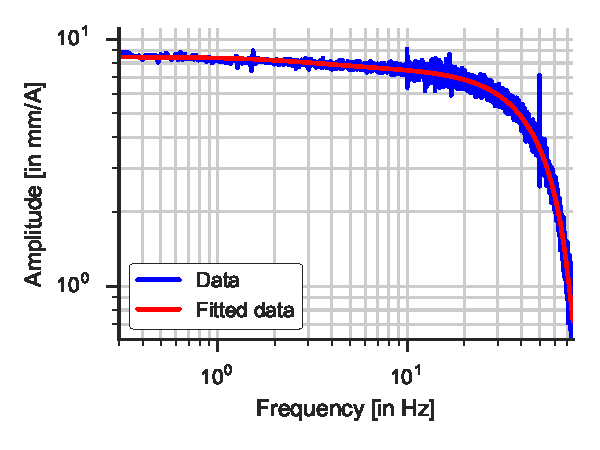
\includegraphics[width=1\linewidth]{img/ctl_id_amplitude}
		\caption{Amplitude}
	\end{subfigure}
	\hfill
	\begin{subfigure}[t]{0.5\linewidth}
		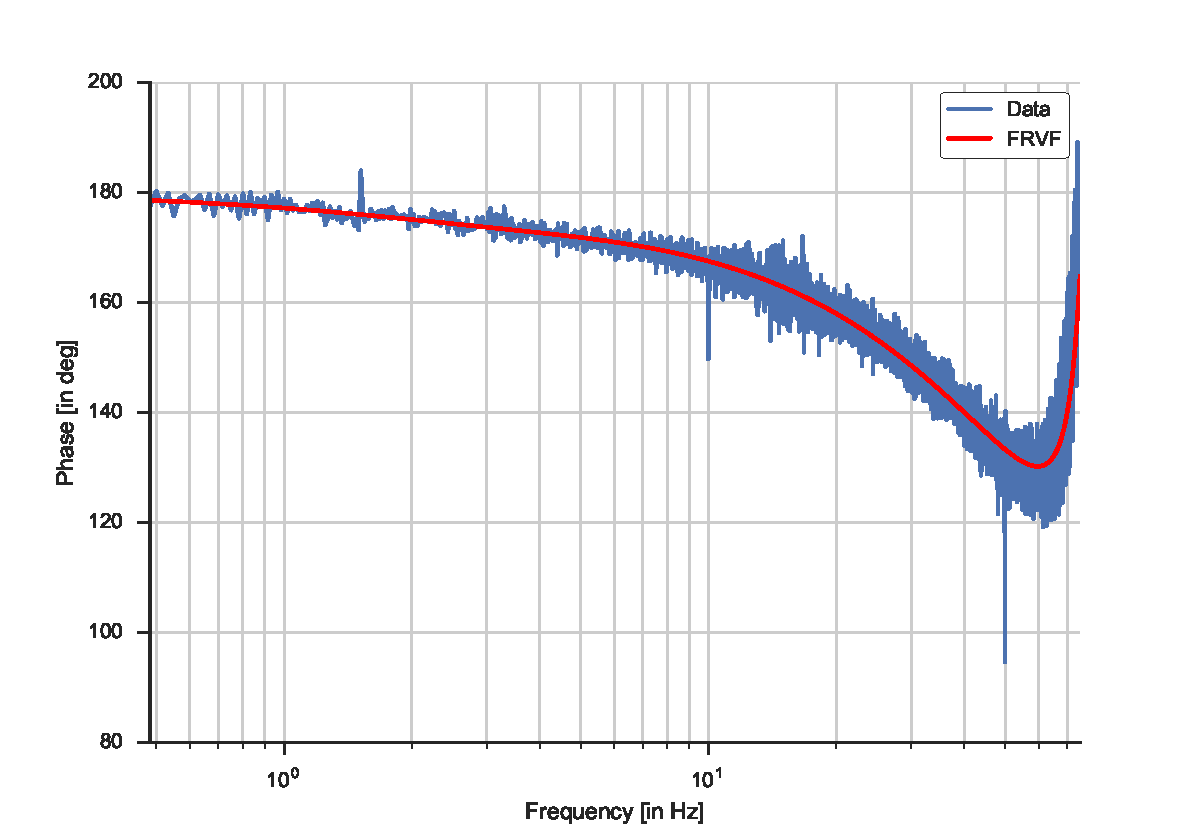
\includegraphics[width=1\linewidth]{img/ctl_id_phase}
		\caption{Phase}
	\end{subfigure}
	\caption{\label{fig:ctl_vfit3}Results of the vector fitting with vfit3}
\end{figure}

It appeared that after converting the system to a transfer function, the numerator was complex. Taking only the real part of each coefficient provided a solution that still fitted the experimental data. In order to obtain a transfer function usable with the response matrix, it was normalized so that its ground gain was 1.

\Cref{fig:ctl_vfit3} shows however only the frequency domain below \SI{75}{\hertz}. In the first simulations, it appeared that the step response presented a large spike which was hardly physically possible (see \cref{fig:ctl_id_spike}). To correct this, the numerator highest degree coefficient was set to 0, which led to the result given in \cref{fig:ctl_id_nospike}. 

\begin{figure}
	\begin{subfigure}[t]{0.5\linewidth}
		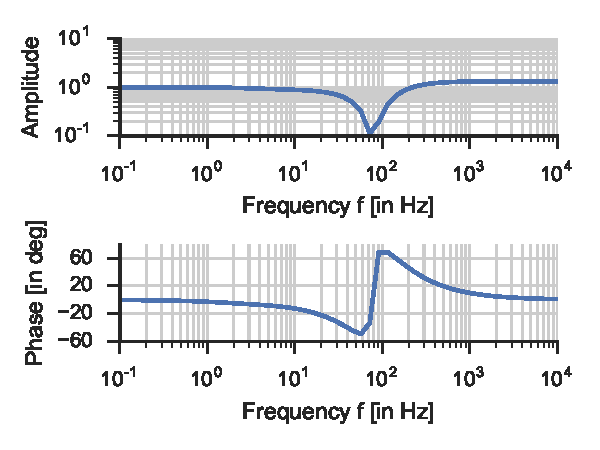
\includegraphics[width=1\linewidth]{img/ctl_id_3z}
		\caption{Frequency response}
	\end{subfigure}
	\hfill
	\begin{subfigure}[t]{0.5\linewidth}
		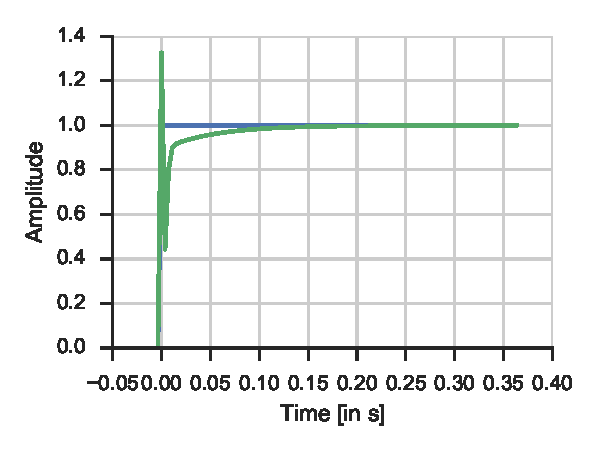
\includegraphics[width=1\linewidth]{img/ctl_id_3z_step}
		\caption{Step response}
	\end{subfigure}
	\caption{\label{fig:ctl_id_spike}Normalized transfer function}
\end{figure}

\begin{figure}
	\begin{subfigure}[t]{0.5\linewidth}
		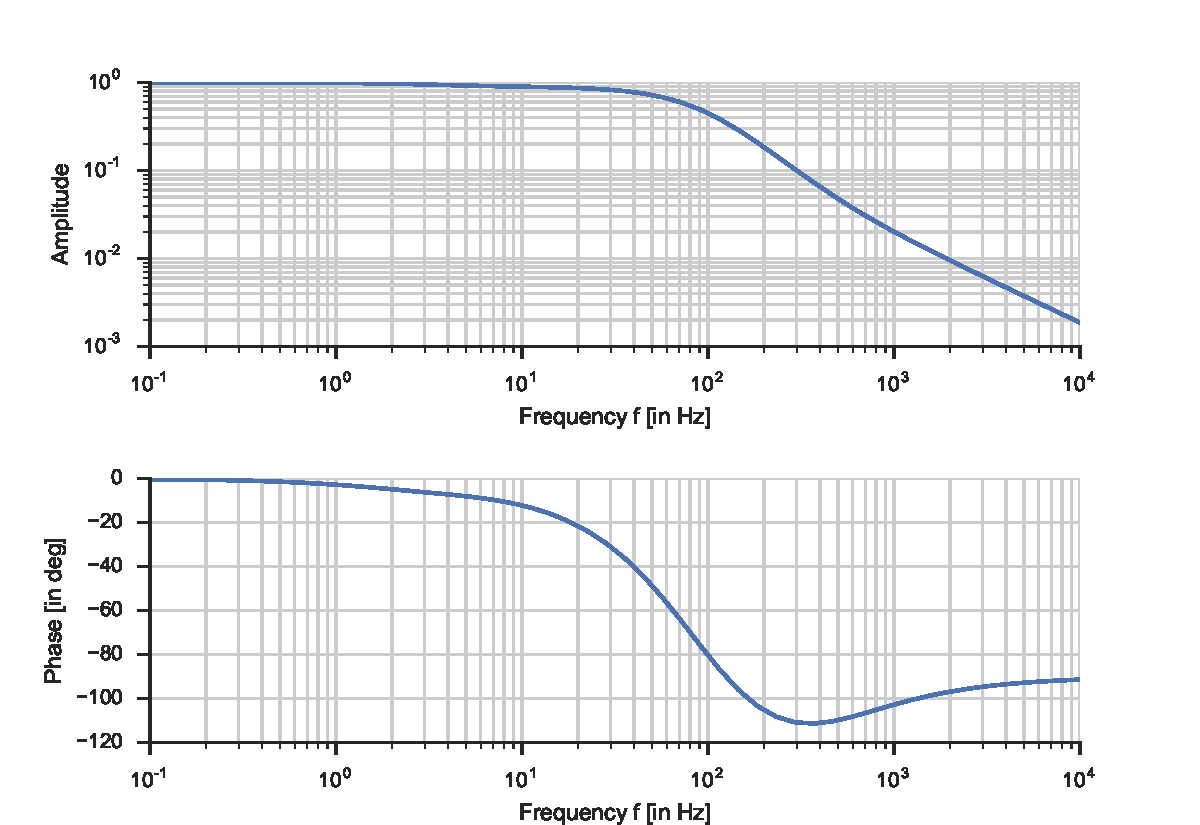
\includegraphics[width=1\linewidth]{img/ctl_id_2z}
		\caption{Frequency response}
	\end{subfigure}
	\hfill
	\begin{subfigure}[t]{0.5\linewidth}
		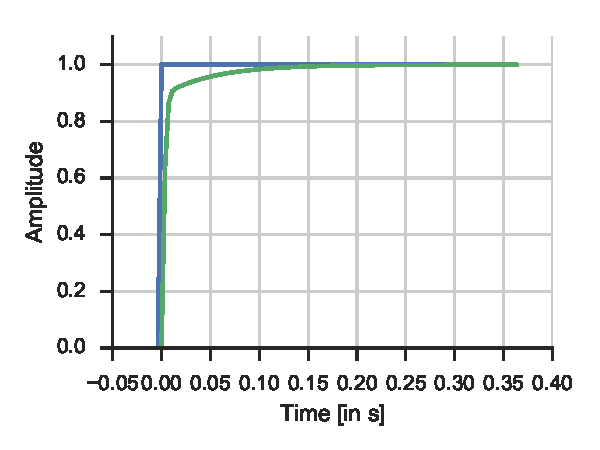
\includegraphics[width=1\linewidth]{img/ctl_id_2z_step}
		\caption{Step response}
	\end{subfigure}
	\caption{\label{fig:ctl_id_nospike}Normalized, zeros-corrected transfer function}
\end{figure}

Finally it the transfer function estimation is 
\begin{equation}
G(s) = \frac{117.322203 \,s^2 + 319144.577 \,s + 6801819.36}
{s^3 + 1171.05630 \,s^2 + 375569.975 \,s +	6801819.36}
\end{equation}

The frequency response given in \cref{fig:ctl_id_nospike} corresponds to what was expected: an amplitude that decreases with frequencies, without amplification domain. To be sure that it corresponds to reality, a simulation of the current situation was conducted.

\section{Simulation model}
\label{sec:correction_simulation}

In order to represent at best the environment, the simulation needs to take into account computation delays and that the correction happens at a given sampled time \SI{150}{\hertz}) whereas other systems perform in continuous time. To achieve that, the simulation is played step by step, at \SI{150}{\hertz} for the correction process and \SI{1.5}{\kilo\hertz} for the continuous time.

\Cref{fig:model_simul} represents the block diagram of the environment, $\text{H}_\text{ring}$ being the identified transfer function of storage ring, and the low pass filter representing the averaging of orbit values in the BPM recording. A initial correction $\vec{\theta}_0$, which is normally provided by a punctual correction process (the slow orbit feedback or SOFB), is needed to ensure the stability of the orbit.

\begin{sidewaysfigure}
    \centering
    \begin{tikzpicture}[auto, node distance=1,>=latex']
%    \draw[help lines, yellow] (-1,-4)grid(15,3);
    \draw [dashed, black] (-.5, 1.7) -- (10.1, 1.7) -- (10.1, -3.5) -- (-.5, -3.5) -- cycle;
    \draw [black](2.8, -3.7) node [above right=0 0.2] {\small mBox --- $F_s=\SI{150}{\hertz}$};

    % We start by placing the blocks
    \node [input] (xref) {};
    \node [operator, right=1.5 of xref] (sum) {$+$};
    \node [operator, right=of sum] (xsmat) {$\times$};
    \node [input, above=of xsmat] (smat) {};
    \node [block, right=of xsmat] (corrector) {K};
    \node [operator, right=of corrector] (suminit) {+};
    \node [input, above=of suminit] (initval) {};
    \node [block, right=of suminit] (DAC) {$\uparrow$};
    \node [block, right=of DAC] (delay) {$\begin{matrix}\text{Delay T}\\\text{\footnotesize Computation}\end{matrix}$};
    \node [operator, right=of delay] (sumperturb) {$+$};
    \node [input, above=of sumperturb] (perturb) {};
    \node [block, right=of sumperturb] (Hring) {$\text{H}_\text{ring}$};
    \node [block, below=of delay] (lowpass) {Low pass};
    \node [block, below=of DAC] (ADC) {$\downarrow$ \SI{150}{\hertz}};
    \coordinate [right= of Hring] (connectout) {};
    \node [input, right= of connectout] (out) {};
    
    % Once the nodes are placed, connecting them is easy.
    \draw [->] (xref)     	-- node [pos=0.2] {$\vec{X}_\text{ref}$} (sum);
    \draw [->] (sum)      	-- node {$\Delta\vec{X}$}    	(xsmat);
    \draw [->] (smat)      	-- node {$\mat{S}*$}    	    (xsmat);
    \draw [->] (xsmat)  	-- node {}                   	(corrector);
    \draw [->] (corrector) 	-- node {$\Delta\vec{\Theta}$} 	(suminit);
    \draw [->] (initval) 	-- node {$\vec{\Theta}_0$}      (suminit);
    \draw [->] (suminit)  	-- node {$\vec{\Theta}$}        (DAC);
    \draw [->] (DAC)      	-- node {}                   	(delay);
    \draw [->] (delay)    	-- node {$\theta(t)$}         	(sumperturb);
    \draw [->] (perturb)  	-- node {$d(t)$}               	(sumperturb);
    \draw [->] (sumperturb) -- node {}                		(Hring);
    \draw [-]  (Hring)    	-- node {}                 		(connectout);
    \draw [->] (connectout) -- node {$x(t)$}          		(out);
    \draw [->] (connectout) |- node {}                 		(lowpass);
    \draw [->] (lowpass)    -- node {}                 		(ADC);
	\draw [->] (ADC)     	-| node[pos=0.5] {$\vec{X}$}
                               node [pos=0.90, left]{$-$}	(sum.south);
    \end{tikzpicture}
    \caption{\label{fig:model_simul}The full model, K being the corrector to define}
\end{sidewaysfigure}

\section{Simulation results}
Several scenarios were designed to validate the simulation, and propose some enhancement to current correction. The delay of the computation is approximated by $\delta t = \SI{3}{\milli\second}$.
 
\subsection{PID correction}
To represent the current configuration in BESSY~II, and validate the model, the PID corrector presented in \cref{sec:correction_state_of_art} was implemented as a pure integrator of amplitude $0.8\cdot \mathrm{F_s}$. The closed-loop system frequency response would be as given in \cref{fig:ctl_freqresp_pid}. As in the reality, frequencies below \SI{10}{\hertz} are damped, and are slightly amplified above. Applying the simulation step by step with a plausible perturbation leads to the result presented in \cref{fig:ctl_sim_pid}.

\begin{figure}
    \centering
    \begin{subfigure}{0.49\textwidth}
        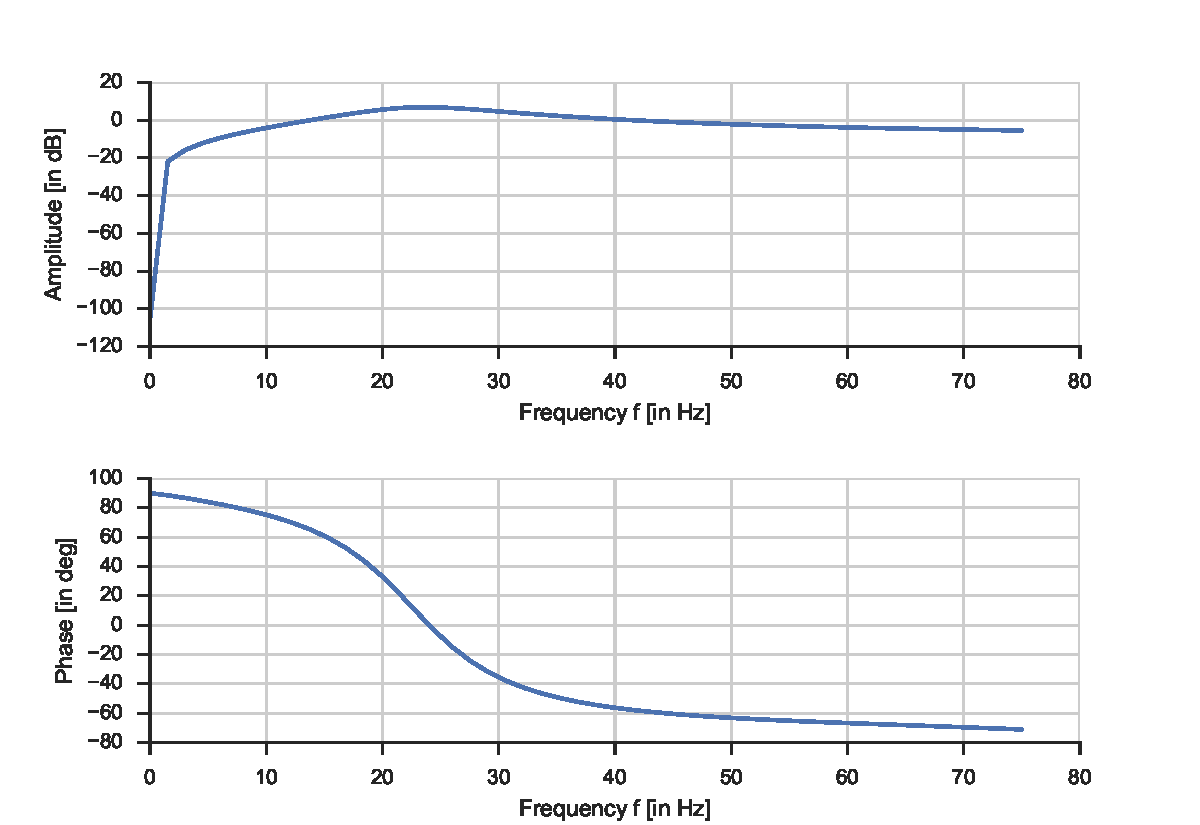
\includegraphics[width=\textwidth]{img/ctl_freqresp_pid}
        \caption{\label{fig:ctl_freqresp_pid} Bode diagram of the closed-loop}
    \end{subfigure}
    \hfill
    \begin{subfigure}{0.49\textwidth}
        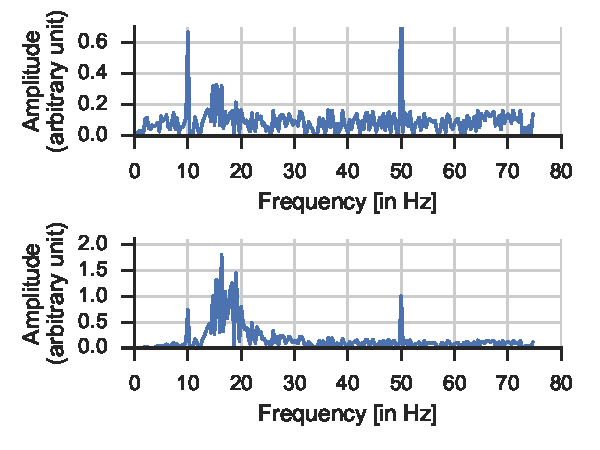
\includegraphics[width=\textwidth]{img/ctl_sim_pid}
        \caption{\label{fig:ctl_sim_pid}Simulation}
        \end{subfigure}    
    \caption{Frequency response for K = PID(0, $0.8\cdot F_s$, 0)}
\end{figure}

The PID can then be slightly enhanced by finding better coefficients, for example with K~=~PID($0.9$, $0.5\cdot\mathrm{F_s}$, $0.15/\mathrm{F_s}$), which result can be seen in \cref{fig:ctl_freqresp_bestpid,fig:ctl_sim_bestpid}. It can be seen there that more frequencies are slightly damped and that the amplified area is smaller, with less gain, providing better results.

\begin{figure}
    \centering
    \begin{subfigure}{0.49\textwidth}
        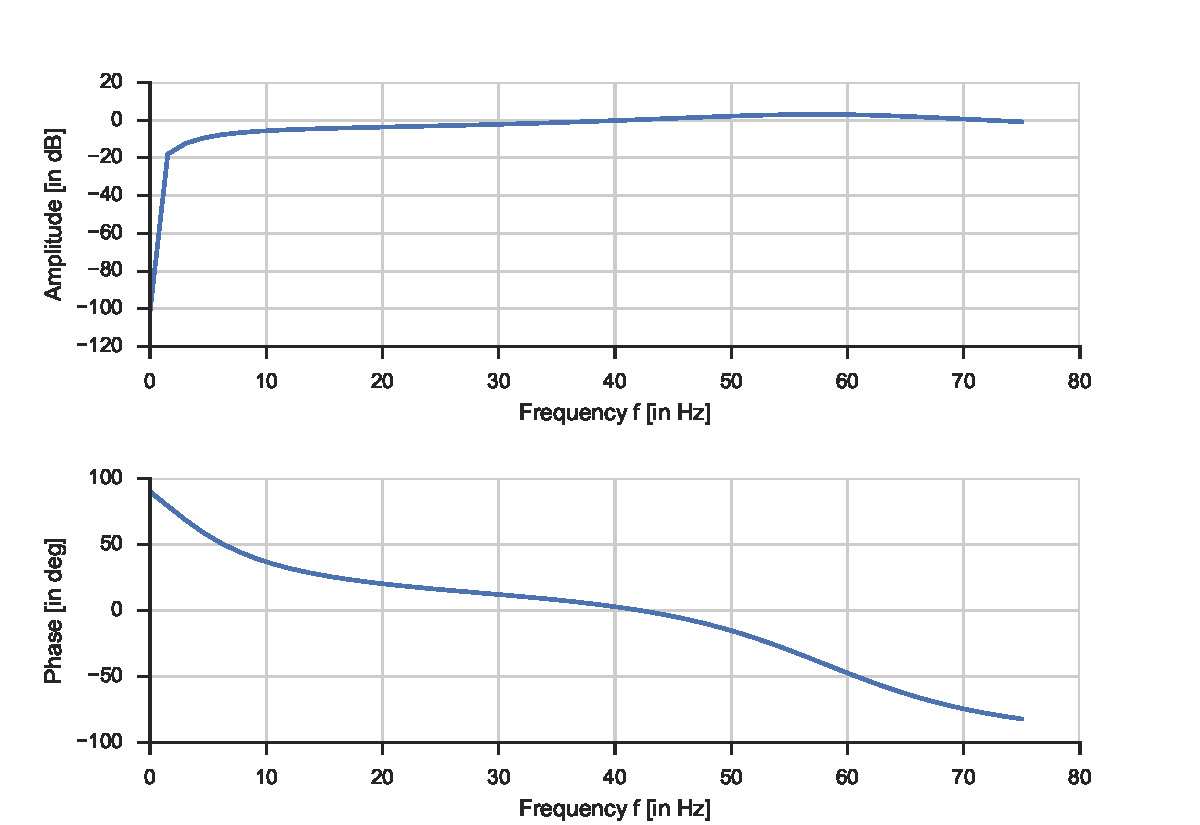
\includegraphics[width=\textwidth]{img/ctl_freqresp_bestpid}
        \caption{\label{fig:ctl_freqresp_bestpid} Bode diagram of the closed-loop}
    \end{subfigure}
    \hfill
    \begin{subfigure}{0.49\textwidth}
        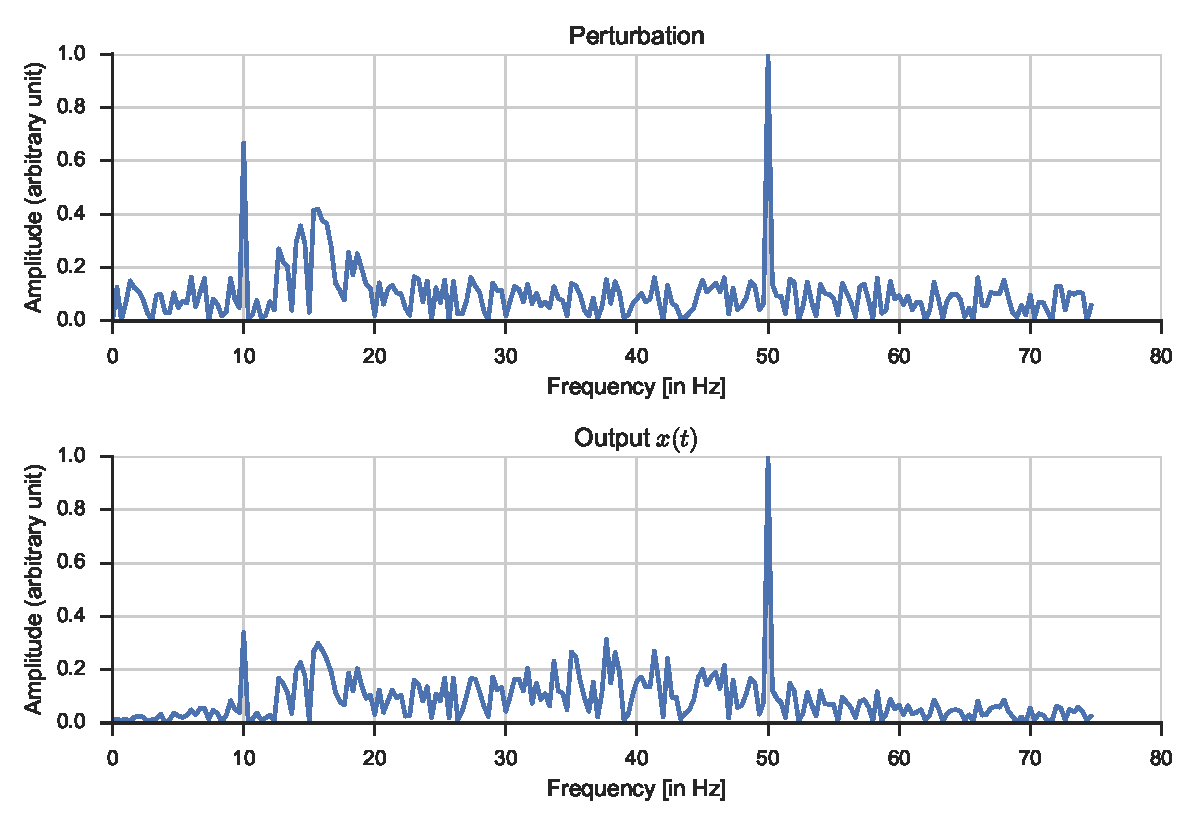
\includegraphics[width=\textwidth]{img/ctl_sim_bestpid}
        \caption{\label{fig:ctl_sim_bestpid}Simulation}
    \end{subfigure}    
    \caption{Frequency response for a better PID}
\end{figure}

\subsection{Optimal correction}
Following the design rules defined in \cite{book:Skogestad-2005}, one can synthesize an $\mathcal{H}_\infty$-corrector, which is an optimal corrector obtained by optimizing the closed and opened loop over the $\infty$-norm\footnote{The $\infty$-norm is defined for vectors as $||\vec{x}||_\infty = \max\limits_{i} |x_i|$} with given parameters. The Robust Control Toolbox from \textsc{Matlab} was used for this effect. The \textsc{Matlab} script given below is an adapted copy of what can be found in Skogestad \cite{book:Skogestad-2005}, page 60. The computation delay is modeled with the Padé approximation of first order \cite{book:matrix} provided by \textsc{Matlab} and added to the system, so that the corrector takes it into account.
\begin{Matlab}
% The robust control toolbox is needed.

% Load ring transfert function
[G_num, G_den] = load(G) 

% Create delay
delay = 0.003;
[dnum, dden] = pade(delay, 1);

G = nd2sys(conv(G_num,d_num),conv(G_den,d_den),1);

% Define parameters
fb = 30  % Bandwidth
wb = fb*2*pi;  
M = 1.001;  % Lim sup (high freq.)
Am = 10^-4;  % Lim sup (low freq.)

% Create weights
Wp = nd2sys([1/M wb], [1 wb*Am]);
Wu = 1;

% Define the system
systemnames = 'G Wp Wu';
inputvar = '[r(1) ; u(1)]';
outputvar = '[Wp; Wu; r-G]';
input_to_G = '[u]';
input_to_Wp = '[r-G]';
input_to_Wu = '[u]';
sysoutname = 'P';
cleanupsysic = 'yes';
sysic;

% Compute corrector
nmeas=1; nu=1; gmn=0.5; gmx=20; tol=0.001;
[khinf,ghinf,gopt] = hinfsyn(P,nmeas,nu,gmn,gmx,tol);
\end{Matlab}

This provides a corrector, which frequency response can be seen in \cref{fig:ctl_freqresp_hinf}: very efficient in low frequencies, it has however an amplification area that can be a problem. Correctors with different bandwidth were synthesized. The simulation is given in \cref{fig:ctl_sim_hinf}. The results are strangely enough always less efficient than the proposed PID (in \cref{fig:ctl_freqresp_bestpid}). \todo{$\mathcal{H}_\infty$: Review this part with Maxim}

\begin{figure}
    \centering
    \begin{subfigure}{0.49\textwidth}
        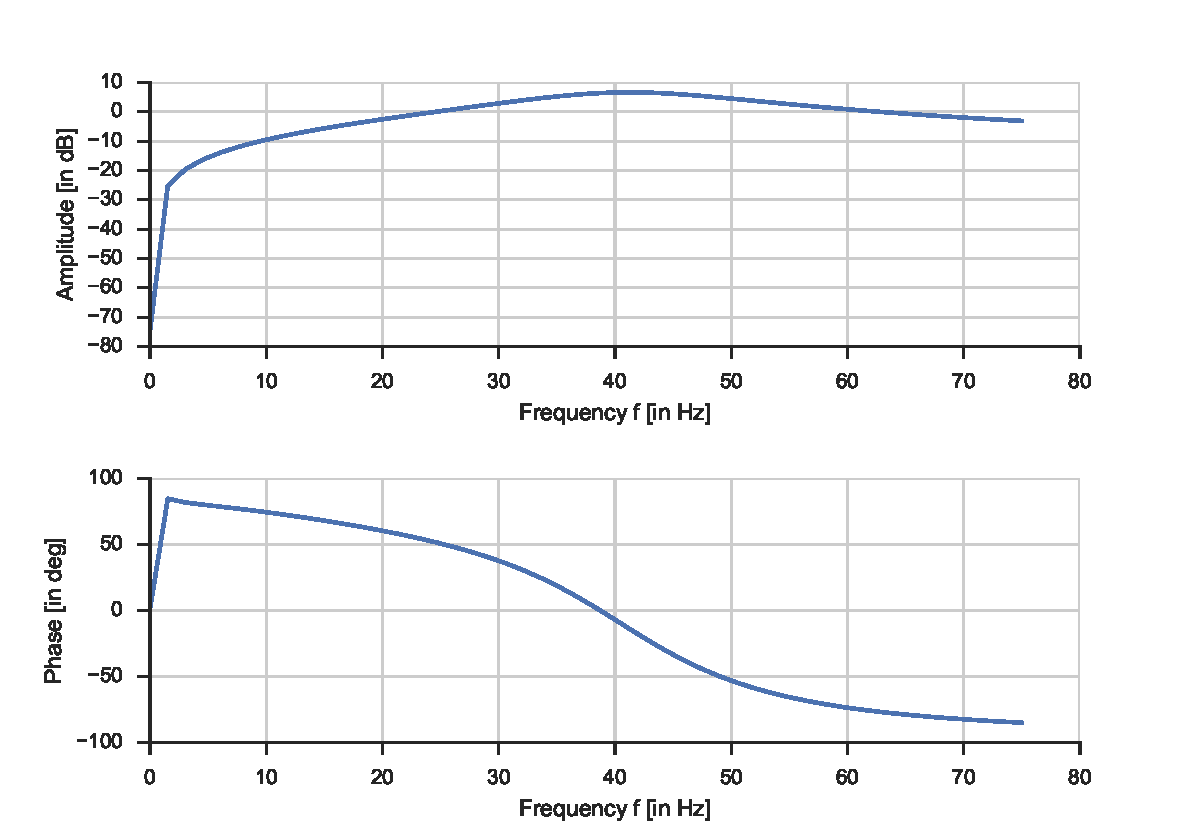
\includegraphics[width=\textwidth]{img/ctl_freqresp_hinf}
        \caption{\label{fig:ctl_freqresp_hinf} Bode diagram of the closed-loop, $f_b$ = \SI{50}{Hz}}
    \end{subfigure}
    \hfill
    \begin{subfigure}{0.49\textwidth}
        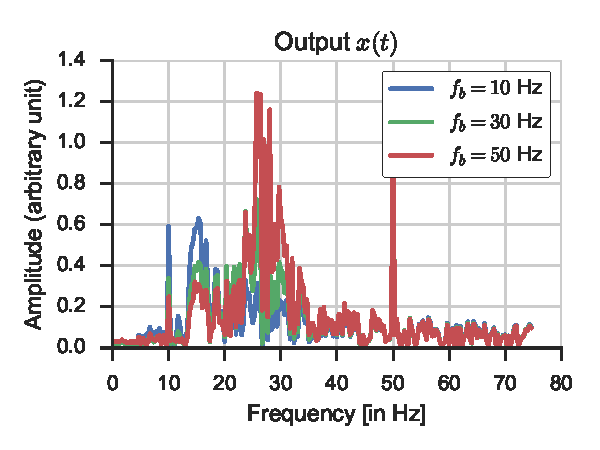
\includegraphics[width=\textwidth]{img/ctl_sim_hinf}
        \caption{\label{fig:ctl_sim_hinf}Simulation (several bandwidths)}
    \end{subfigure}    
    \caption{Frequency response of $\mathcal{H}_\infty$-correctors}
\end{figure}

\section{Summary}
A simulation environment was built in order to be able to predict the influence of some parameters on the system and to closely study how to correct at best the orbit position.

A first system approximation was identified from the ring. From this was predicted that a more optimized PID corrector is possible, which only needs to be validated experimentally.  \todo{Un mot sur la correction optimale}The optimal correction direction must be considered in more depth and, on a more ambitious perspective, the design of robust MIMO correctors would certainly provide better and more reliable results.